\documentclass[12pt]{article}

% Idioma e codificação
\usepackage[brazil]{babel}
\usepackage[utf8]{inputenc}
\usepackage[T1]{fontenc}

% Matemática e listas
\usepackage{amsmath, amssymb}
\usepackage{enumitem}

% Layout e cores
\usepackage{geometry}
\usepackage{graphicx}
\usepackage{xcolor}

% Cores institucionais
\definecolor{maincolor}{RGB}{0, 79, 151}
\definecolor{meuazul}{RGB}{0, 79, 151}

% Cabeçalho e rodapé
\usepackage{fancyhdr}

% Blocos
\usepackage[most]{tcolorbox}
\newtcolorbox{block}[1]{%
  colback=blue!5,
  colframe=maincolor,
  coltitle=white,
  title=#1,
  fonttitle=\bfseries,
  boxrule=1.5pt,
  arc=3mm,
  left=6pt,
  right=6pt,
  top=6pt,
  bottom=6pt,
  breakable
}

\newtcolorbox{resposta}[1]{%
  colback=white,
  colframe=meuazul!30,
  arc=1mm,
  height=#1,
  width=\textwidth,
  boxrule=0.8pt
}

% Margens
\geometry{margin=2.5cm}

% Fancyhdr
\pagestyle{fancy}
\fancyhf{}

\renewcommand{\headrulewidth}{2pt}
\renewcommand{\footrulewidth}{2pt}

\renewcommand{\headrule}{\hbox to\headwidth{%
  \color{meuazul}\leaders\hrule height \headrulewidth\hfill}}

\renewcommand{\footrule}{\hbox to\headwidth{%
  \color{meuazul}\leaders\hrule height \footrulewidth\hfill}}

\setlength{\headheight}{52pt}
\addtolength{\topmargin}{-20pt}

\fancyhead[L]{%
  
\includegraphics[height=1.2cm]{logo.png}
}

\fancyhead[R]{%
  \raggedleft
  \textcolor{meuazul}{%
    \small
    \textbf{Exercício de Normalização — Banco de Dados I}\\
    Me.~Sergio Souza Novak\\
    \textit{Sistemas de Informação / Engenharia de Software}
  }
}

\fancyfoot[C]{\textcolor{meuazul}{\thepage}}

% =========================
\begin{document}
% =========================

\vspace*{0.2cm}

\begin{center}
  {\Large \textbf{Exercício de Normalização de Banco de Dados e Lingugagem SQL comandos DDL}}\\[0.2cm]
  \textit{Instruções: Analise os diagramas fornecidos e responda as questões sobre as formas normais.
  Justifique suas respostas com base nos conceitos de dependência funcional.}
\end{center}

\vspace{0.4cm}

\begin{block}{Conceitos de Referência}
  \small
  \begin{itemize}
    \item \textbf{1FN}: Atributos atômicos e ausência de grupos repetitivos.
    \item \textbf{2FN}: Deve estar na 1FN e os atributos não-chave devem depender totalmente da chave primária (sem dependências parciais).
    \item \textbf{3FN}: Deve estar na 2FN e os atributos não-chave não podem depender de outros atributos não-chave (sem dependências transitivas).
  \end{itemize}
\end{block}

\vspace{0.5cm}

% -------------------------------------------------------
% QUESTÃO 1
% -------------------------------------------------------
\textbf{1.} Observe o diagrama abaixo representando o estado inicial do banco de dados (\textbf{1FN}):

\begin{center}
  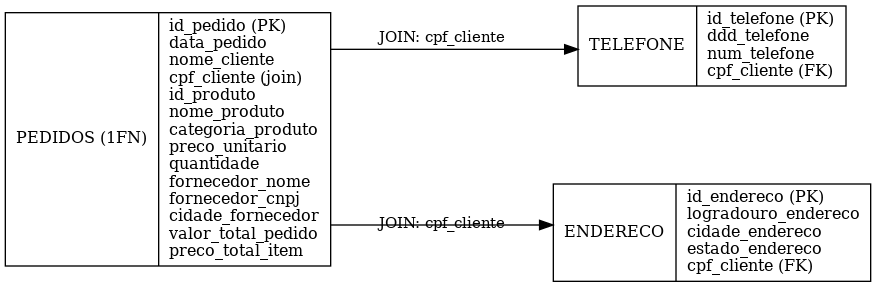
\includegraphics[width=0.9\textwidth]{1FN.png}
\end{center}

\begin{enumerate}[label=\alph*)]
  \item Analisando a tabela \textbf{PEDIDOS (1FN)}, identifique quais atributos dependem apenas de parte da chave composta (se considerarmos \textit{id\_pedido} e \textit{id\_produto} como chave).
  \item Por que a separação das tabelas \textbf{TELEFONE} e \textbf{ENDERECO} é necessária para satisfazer a 1FN?
\end{enumerate}
\begin{resposta}{4.5cm}
\end{resposta}



% -------------------------------------------------------
% QUESTÃO 2
% -------------------------------------------------------
\textbf{2.} Analise o diagrama em \textbf{Segunda Forma Normal (2FN)}:

\begin{center}
  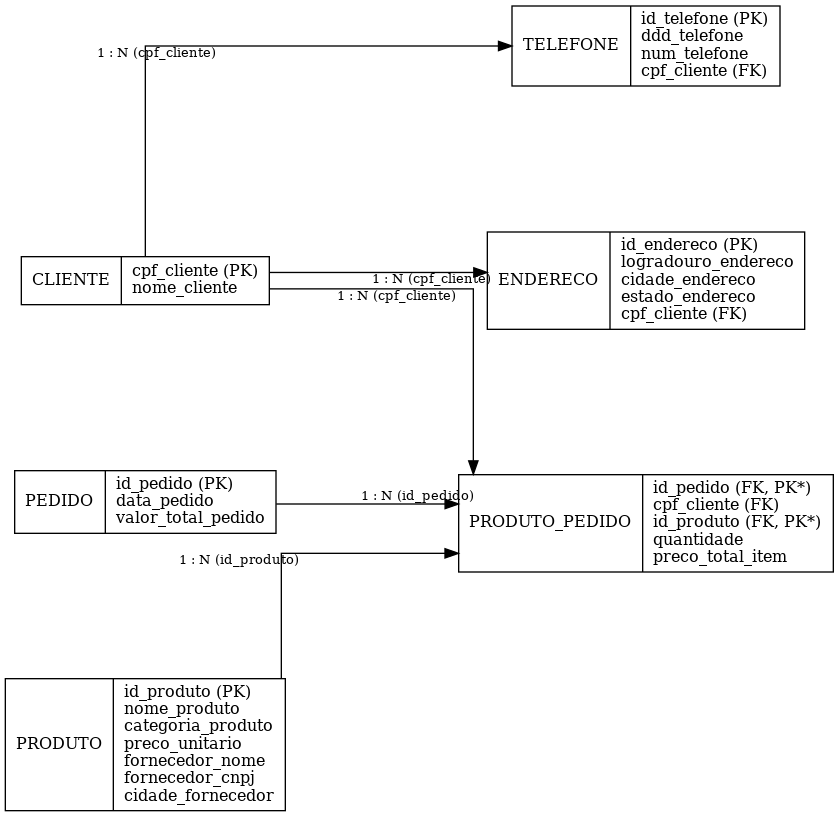
\includegraphics[width=0.7\textwidth]{2FN.png}
\end{center}

\begin{enumerate}[label=\alph*)]
  \item Como a criação da tabela \textbf{PRODUTO\_PEDIDO} ajudou a resolver o problema das dependências parciais encontradas no diagrama anterior?
  \item No diagrama acima, ainda existe alguma redundância relacionada aos dados do \textbf{Fornecedor}? Justifique.
\end{enumerate}
\begin{resposta}{6cm}
\end{resposta}



% -------------------------------------------------------
% QUESTÃO 3
% -------------------------------------------------------
\textbf{3.} Finalmente, observe o diagrama em \textbf{Terceira Forma Normal (3FN)}:

\begin{center}
  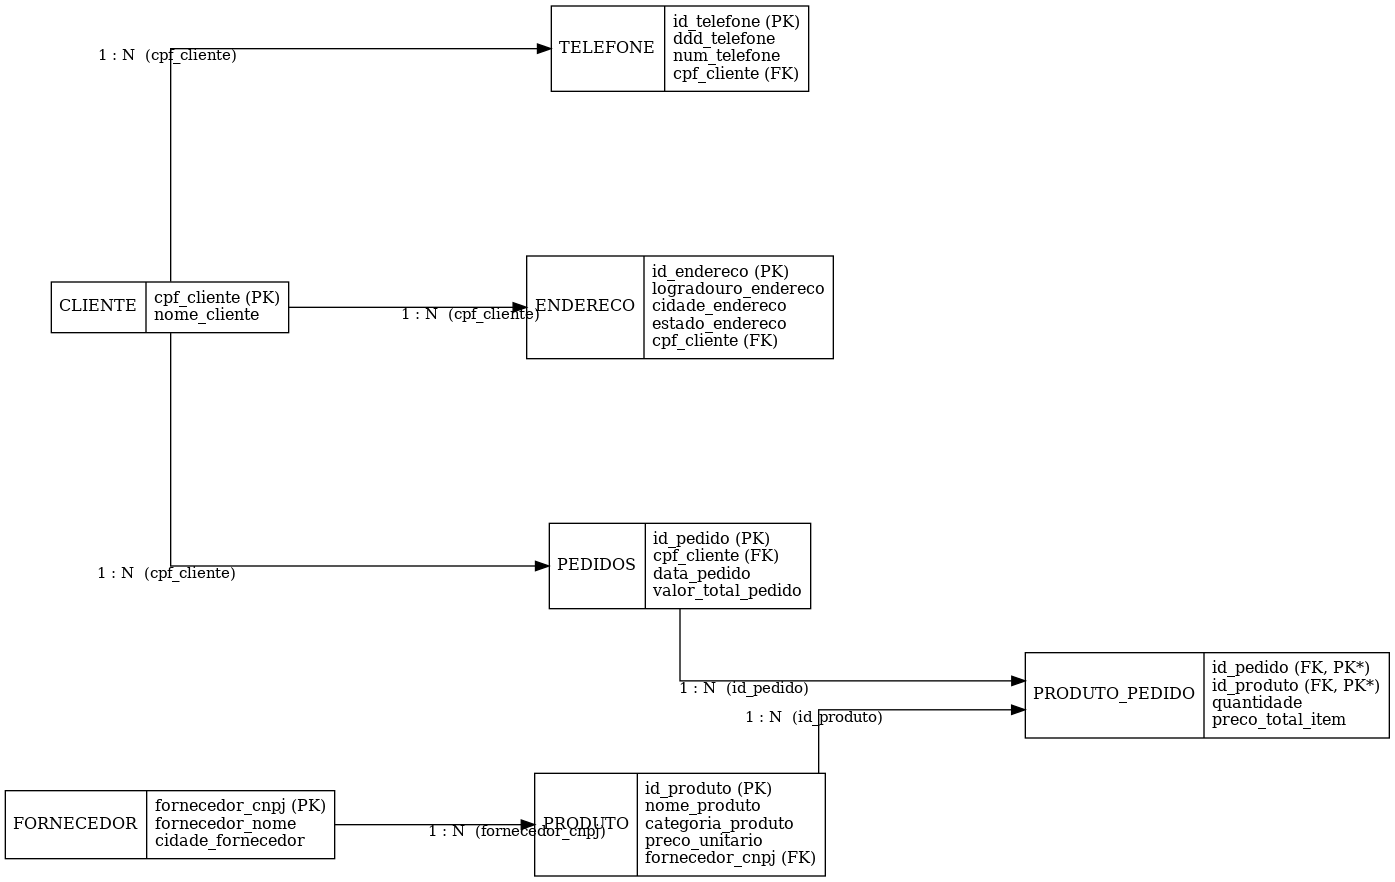
\includegraphics[width=\textwidth]{3FN.png}
\end{center}

\begin{enumerate}[label=\alph*)]
  \item Explique por que a criação da tabela \textbf{FORNECEDOR} foi necessária para atingir a 3FN. Qual era a \textbf{dependência transitiva} existente no diagrama anterior?
  \item Descreva a vantagem de se ter o banco de dados nesta estrutura final em termos de manutenção e integridade dos dados.
\end{enumerate}
\begin{resposta}{7cm}
\end{resposta}


\begin{block}{Trecho de Código SQL (Simplificado)}
\footnotesize
\begin{verbatim}
-- =========================
-- DROP (ordem segura)
-- =========================
DROP TABLE IF EXISTS 
    Funcionario_Supervisor,
    Proprietario_Equipamento,
    Ordenha_Equipamento,
    Ordenha_Supervisor,
    Ordenha_Funcionario,
    Vaca_Veterinario,
    Ordenha,
    Vaca,
    Equipamentos,
    Veterinario,
    Funcionario,
    Supervisor,
    Proprietario
CASCADE;

-- =========================
-- TABELAS PRINCIPAIS
-- =========================

CREATE TABLE Proprietario (
    id SERIAL PRIMARY KEY,
    nome_completo VARCHAR(100),
    telefone VARCHAR(20)
);

CREATE TABLE Equipamentos (
    codigo_equipamento SERIAL PRIMARY KEY,
    tipo VARCHAR(50),
    ultima_manutencao DATE,
    situacao VARCHAR(50)
);

CREATE TABLE Vaca (
    id SERIAL PRIMARY KEY,
    data_nascimento DATE,
    raca VARCHAR(50),
    peso DECIMAL(6,2),
    status_saude VARCHAR(50)
);

CREATE TABLE Veterinario (
    id SERIAL PRIMARY KEY,
    nome_completo VARCHAR(100),
    telefone VARCHAR(20),
    registro_profissional VARCHAR(50)
);

CREATE TABLE Funcionario (
    id SERIAL PRIMARY KEY,
    nome_completo VARCHAR(100),
    telefone VARCHAR(20),
    turno_periodo VARCHAR(50)
);

CREATE TABLE Supervisor (
    id SERIAL PRIMARY KEY,
    nome_completo VARCHAR(100),
    telefone VARCHAR(20),
    turno_supervisao VARCHAR(50)
);

CREATE TABLE Ordenha (
    id SERIAL PRIMARY KEY,
    data DATE,
    horario TIME,
    quantidade_leite DECIMAL(6,2),
    id_proprietario INT,
    id_vaca INT NOT NULL
);

-- =========================
-- CHAVES ESTRANGEIRAS (1:N)
-- =========================

ALTER TABLE Ordenha 
ADD CONSTRAINT fk_ordenha_proprietario 
FOREIGN KEY (id_proprietario) REFERENCES Proprietario(id);

ALTER TABLE Ordenha 
ADD CONSTRAINT fk_ordenha_vaca 
FOREIGN KEY (id_vaca) REFERENCES Vaca(id);

-- =========================
-- RELACIONAMENTOS N:N
-- =========================

-- Vaca <-> Veterinario
CREATE TABLE Vaca_Veterinario (
    id_veterinario INT NOT NULL,
    id_vaca INT NOT NULL,
    PRIMARY KEY (id_veterinario, id_vaca),
    FOREIGN KEY (id_veterinario) REFERENCES Veterinario(id),
    FOREIGN KEY (id_vaca) REFERENCES Vaca(id)
);

-- Ordenha <-> Funcionario
CREATE TABLE Ordenha_Funcionario (
    id_ordenha INT NOT NULL,
    id_funcionario INT NOT NULL,
    PRIMARY KEY (id_ordenha, id_funcionario),
    FOREIGN KEY (id_ordenha) REFERENCES Ordenha(id),
    FOREIGN KEY (id_funcionario) REFERENCES Funcionario(id)
);

-- Ordenha <-> Supervisor
CREATE TABLE Ordenha_Supervisor (
    id_ordenha INT NOT NULL,
    id_supervisor INT NOT NULL,
    PRIMARY KEY (id_ordenha, id_supervisor),
    FOREIGN KEY (id_ordenha) REFERENCES Ordenha(id),
    FOREIGN KEY (id_supervisor) REFERENCES Supervisor(id)
);

-- Ordenha <-> Equipamentos
CREATE TABLE Ordenha_Equipamento (
    id_ordenha INT NOT NULL,
    codigo_equipamento INT NOT NULL,
    PRIMARY KEY (id_ordenha, codigo_equipamento),
    FOREIGN KEY (id_ordenha) REFERENCES Ordenha(id),
    FOREIGN KEY (codigo_equipamento) REFERENCES Equipamentos(codigo_equipamento)
);

-- Proprietario <-> Equipamentos
CREATE TABLE Proprietario_Equipamento (
    id_proprietario INT NOT NULL,
    codigo_equipamento INT NOT NULL,
    PRIMARY KEY (id_proprietario, codigo_equipamento),
    FOREIGN KEY (id_proprietario) REFERENCES Proprietario(id),
    FOREIGN KEY (codigo_equipamento) REFERENCES Equipamentos(codigo_equipamento)
);

-- Funcionario <-> Supervisor
CREATE TABLE Funcionario_Supervisor (
    id_funcionario INT NOT NULL,
    id_supervisor INT NOT NULL,
    PRIMARY KEY (id_funcionario, id_supervisor),
    FOREIGN KEY (id_funcionario) REFERENCES Funcionario(id),
    FOREIGN KEY (id_supervisor) REFERENCES Supervisor(id)
);



-- =========================
-- 1. TABELAS PRINCIPAIS
-- =========================

-- Proprietarios
INSERT INTO Proprietario (nome_completo, telefone) VALUES
('João Silva', '62999990001'),
('Maria Souza', '62999990002'),
('Carlos Pereira', '62999990003');

-- Equipamentos
INSERT INTO Equipamentos (tipo, ultima_manutencao, situacao) VALUES
('Ordenhadeira', '2026-03-01', 'Ativo'),
('Resfriador', '2026-02-15', 'Ativo'),
('Bomba de Leite', '2026-01-10', 'Manutenção');

-- Vacas
INSERT INTO Vaca (data_nascimento, raca, peso, status_saude) VALUES
('2020-05-10', 'Holandesa', 550.00, 'Saudável'),
('2019-08-20', 'Jersey', 480.00, 'Saudável'),
('2021-02-15', 'Gir', 520.00, 'Tratamento');

-- Veterinarios
INSERT INTO Veterinario (nome_completo, telefone, registro_profissional) VALUES
('Dr. Carlos Lima', '62988880001', 'CRMV123'),
('Dra. Ana Paula', '62988880002', 'CRMV456');

-- Funcionarios
INSERT INTO Funcionario (nome_completo, telefone, turno_periodo) VALUES
('Pedro Santos', '62977770001', 'Manhã'),
('Lucas Oliveira', '62977770002', 'Tarde'),
('Bruno Alves', '62977770003', 'Noite');

-- Supervisores
INSERT INTO Supervisor (nome_completo, telefone, turno_supervisao) VALUES
('Marcos Silva', '62966660001', 'Manhã'),
('Fernanda Costa', '62966660002', 'Noite');

-- =========================
-- 2. ORDENHA (1:N)
-- =========================

INSERT INTO Ordenha (data, horario, quantidade_leite, id_proprietario, id_vaca) VALUES
('2026-04-10', '06:00', 25.5, 1, 1),
('2026-04-10', '18:00', 27.0, 1, 2),
('2026-04-11', '06:00', 26.3, 2, 1),
('2026-04-11', '18:00', 24.8, 3, 3);

-- =========================
-- 3. RELACIONAMENTOS N:N
-- =========================

-- Vaca <-> Veterinario
INSERT INTO Vaca_Veterinario (id_veterinario, id_vaca) VALUES
(1,1),
(1,2),
(2,3),
(2,1);

-- Ordenha <-> Funcionario
INSERT INTO Ordenha_Funcionario (id_ordenha, id_funcionario) VALUES
(1,1),
(1,2),
(2,1),
(3,2),
(4,3);

-- Ordenha <-> Supervisor
INSERT INTO Ordenha_Supervisor (id_ordenha, id_supervisor) VALUES
(1,1),
(2,1),
(3,2),
(4,2);

-- Ordenha <-> Equipamentos
INSERT INTO Ordenha_Equipamento (id_ordenha, codigo_equipamento) VALUES
(1,1),
(1,2),
(2,1),
(3,2),
(4,3);

-- Proprietario <-> Equipamentos
INSERT INTO Proprietario_Equipamento (id_proprietario, codigo_equipamento) VALUES
(1,1),
(1,2),
(2,2),
(3,3);

-- Funcionario <-> Supervisor
INSERT INTO Funcionario_Supervisor (id_funcionario, id_supervisor) VALUES
(1,1),
(2,1),
(2,2),
(3,2);
\end{verbatim}
\end{block}

\vspace{0.4cm}

% -------------------------------------------------------
% QUESTÃO 4
% -------------------------------------------------------
\textbf{4.} No código acima, observe a tabela \textbf{Ordenha}.
\begin{enumerate}[label=\alph*)]
  \item Qual é o tipo de relacionamento entre a tabela \textbf{Vaca} e a tabela \textbf{Ordenha}? (Ex: 1:1, 1:N ou N:N). Justifique sua resposta com base na chave estrangeira.
  \item O que aconteceria se tentássemos excluir uma \textbf{Vaca} que já possui registros de \textbf{Ordenha} vinculados a ela?
\end{enumerate}
\begin{resposta}{4.5cm}
\end{resposta}



% -------------------------------------------------------
% QUESTÃO 5
% -------------------------------------------------------
\textbf{5.} Analise a estrutura da tabela \textbf{Vaca\_Veterinario}.
\begin{enumerate}[label=\alph*)]
  \item Por que esta tabela possui uma \textbf{Chave Primária Composta}? O que isso representa no mundo real em termos de atendimento veterinário?
  \item Qual a diferença fundamental de cardinalidade entre este relacionamento e o relacionamento entre \textbf{Vaca} e \textbf{Ordenha}?
\end{enumerate}
\begin{resposta}{5cm}
\end{resposta}

\vspace{0.5cm}

% -------------------------------------------------------
% QUESTÃO 6
% -------------------------------------------------------
\textbf{6.} No arquivo original, existia o comando \texttt{DROP TABLE IF EXISTS ... CASCADE;}.
\begin{enumerate}[label=\alph*)]
  \item Explique a função da palavra-chave \textbf{CASCADE} neste contexto.
  \item Por que é considerada uma "boa prática" (em scripts de desenvolvimento) listar as tabelas de relacionamento (como \textit{Ordenha\_Funcionario}) antes das tabelas principais (como \textit{Funcionario}) no comando \texttt{DROP}?
\end{enumerate}
\begin{resposta}{5cm}
\end{resposta}

\vspace{0.5cm}

% -------------------------------------------------------
% QUESTÃO 7
% -------------------------------------------------------
\textbf{7.} Considere o seguinte comando de inserção: 
\texttt{INSERT INTO Ordenha (data, horario, quantidade\_leite, id\_vaca) VALUES ('2026-04-10', '06:00', 25.5, 999);}
\begin{enumerate}[label=\alph*)]
  \item Supondo que não exista nenhuma vaca com o \texttt{id = 999}, o banco de dados aceitará essa inserção? Justifique mencionando o conceito de \textbf{Integridade Referencial}.
  \item Como o uso do tipo \textbf{SERIAL} na Chave Primária auxilia o desenvolvedor durante a inserção de novos registros?
\end{enumerate}
\begin{resposta}{5cm}
\end{resposta}

\vspace{0.5cm}

% -------------------------------------------------------
% QUESTÃO 8
% -------------------------------------------------------
\textbf{8.} No código fornecido, as chaves estrangeiras da tabela \textbf{Ordenha} foram adicionadas posteriormente utilizando o comando \texttt{ALTER TABLE}.
\begin{enumerate}[label=\alph*)]
  \item Reescreva o comando \texttt{CREATE TABLE Ordenha} de modo que as chaves estrangeiras (\textit{id\_proprietario} e \textit{id\_vaca}) sejam definidas diretamente dentro da criação da tabela, dispensando o uso de \texttt{ALTER TABLE}.
  \item Qual a vantagem pedagógica ou organizacional de se definir as constraints diretamente no \texttt{CREATE TABLE} em relação ao \texttt{ALTER TABLE}?
\end{enumerate}
\begin{resposta}{6cm}
\end{resposta}

\vspace{0.8cm}



\begin{block}{Esquema SQL: Empregados e Companhias}
\footnotesize
\begin{verbatim}


-- =========================
-- DROP (ordem segura)
-- =========================
DROP TABLE IF EXISTS 
    tbTrabalha,
    tbEmpregado,
    tbCompanhia,
    tbGerente
CASCADE;

-- =========================
-- TABELAS PRINCIPAIS
-- =========================

-- Gerente
CREATE TABLE tbGerente (
    cod_gerente SERIAL PRIMARY KEY,
    nome_gerente VARCHAR(100)
);

-- Companhia
CREATE TABLE tbCompanhia (
    cod_companhia SERIAL PRIMARY KEY,
    nome_companhia VARCHAR(100),
    cidade_companhia VARCHAR(100)
);

-- Empregado
CREATE TABLE tbEmpregado (
    cod_emp SERIAL PRIMARY KEY,
    nome_emp VARCHAR(100),
    rua_emp VARCHAR(100),
    cidade_emp VARCHAR(100),
    fone_emp VARCHAR(20),
    cod_gerente INT
);

-- Trabalha (N:N com atributo salário)
CREATE TABLE tbTrabalha (
    cod_emp INT NOT NULL,
    cod_companhia INT NOT NULL,
    salario DECIMAL(10,2),
    PRIMARY KEY (cod_emp, cod_companhia)
);

-- =========================
-- CHAVES ESTRANGEIRAS
-- =========================

-- Empregado -> Gerente
ALTER TABLE tbEmpregado
ADD CONSTRAINT fk_empregado_gerente
FOREIGN KEY (cod_gerente)
REFERENCES tbGerente(cod_gerente);

-- Trabalha -> Empregado
ALTER TABLE tbTrabalha
ADD CONSTRAINT fk_trabalha_empregado
FOREIGN KEY (cod_emp)
REFERENCES tbEmpregado(cod_emp);

-- Trabalha -> Companhia
ALTER TABLE tbTrabalha
ADD CONSTRAINT fk_trabalha_companhia
FOREIGN KEY (cod_companhia)
REFERENCES tbCompanhia(cod_companhia);

-- =========================
-- INSERTS
-- =========================

-- Gerentes
INSERT INTO tbGerente (nome_gerente) VALUES
('Carlos Mendes'),
('Fernanda Alves'),
('Roberto Lima');

-- Companhias
INSERT INTO tbCompanhia (nome_companhia, cidade_companhia) VALUES
('Tech Solutions', 'Goiânia'),
('AgroTech', 'Anápolis'),
('DataCorp', 'Brasília');

-- Empregados
INSERT INTO tbEmpregado (nome_emp, rua_emp, cidade_emp, fone_emp, cod_gerente) VALUES
('João Silva', 'Rua A', 'Goiânia', '62999990001', 1),
('Maria Souza', 'Rua B', 'Goiânia', '62999990002', 1),
('Pedro Santos', 'Rua C', 'Anápolis', '62999990003', 2),
('Ana Costa', 'Rua D', 'Brasília', '61999990004', 3);

-- Trabalha
INSERT INTO tbTrabalha (cod_emp, cod_companhia, salario) VALUES
(1,1,3500.00),
(1,2,3800.00),
(2,1,3200.00),
(3,2,4000.00),
(4,3,4500.00);
\end{verbatim}
\end{block}

\vspace{0.4cm}

% -------------------------------------------------------
% QUESTÃO 9
% -------------------------------------------------------
\textbf{9.} Analisando a tabela \textbf{tbTrabalha}:
\begin{enumerate}[label=\alph*)]
  \item Por que ela possui uma chave primária composta? 
  \item Explique por que o atributo \textbf{salario} está localizado nesta tabela e não em \textbf{tbEmpregado}.
\end{enumerate}
\begin{resposta}{4cm}
\end{resposta}

\vspace{0.5cm}

% -------------------------------------------------------
% QUESTÃO 10
% -------------------------------------------------------
\textbf{10.} Identifique o tipo de relacionamento (Ex: 1:1, 1:N, N:N) entre:
\begin{enumerate}[label=\alph*)]
  \item \textbf{tbGerente} e \textbf{tbEmpregado}: 
  \item \textbf{tbEmpregado} e \textbf{tbCompanhia}:
\end{enumerate}
\begin{resposta}{3cm}
\end{resposta}

\vspace{0.5cm}

% -------------------------------------------------------
% QUESTÃO 11
% -------------------------------------------------------
\textbf{11.} Sobre Normalização:
\begin{enumerate}[label=\alph*)]
  \item A tabela \textbf{tbEmpregado} apresenta alguma dependência que viole a 2FN ou 3FN? Justifique.
  \item Se decidíssemos armazenar o CEP e o bairro do empregado, como deveríamos estruturar essas tabelas para garantir a 3FN?
\end{enumerate}
\begin{resposta}{4.5cm}
\end{resposta}



% -------------------------------------------------------
% QUESTÃO 12
% -------------------------------------------------------
\textbf{12.} Com base nos dados inseridos, o empregado \textbf{João Silva} (cod\_emp = 1) possui registros em quantas companhias? O que isso demonstra sobre a flexibilidade do modelo N:N?
\begin{resposta}{4cm}
\end{resposta}

\vspace{0.5cm}

% -------------------------------------------------------
% QUESTÃO 13
% -------------------------------------------------------
\textbf{13.} Escreva um comando SQL (DQL) que retorne o \textbf{nome do empregado} e o \textbf{nome do seu gerente} correspondente, realizando o JOIN adequado.
\begin{resposta}{4.5cm}
\end{resposta}

\vspace{0.5cm}

% -------------------------------------------------------
% QUESTÃO 14
% -------------------------------------------------------
\textbf{14.} Como poderíamos alterar a tabela \textbf{tbTrabalha} para garantir que o salário nunca seja um valor negativo? Escreva o comando de \texttt{ALTER TABLE} com uma \texttt{CHECK CONSTRAINT}.
\begin{resposta}{4cm}
\end{resposta}

\vspace{0.5cm}

% -------------------------------------------------------
% QUESTÃO 15
% -------------------------------------------------------
\textbf{15.} Escreva uma consulta SQL que retorne a \textbf{média salarial} dos funcionários que trabalham na companhia 'Tech Solutions'.
\begin{resposta}{4.5cm}
\end{resposta}



% -------------------------------------------------------
% QUESTÃO 16
% -------------------------------------------------------
\textbf{16.} Se deletarmos o registro do gerente 'Carlos Mendes' (cod\_gerente = 1), o que ocorrerá com os registros de 'João Silva' e 'Maria Souza' na tabela \textbf{tbEmpregado}? Explique o conceito de Restrição de Integridade envolvido.
\begin{resposta}{5cm}
\end{resposta}

\vspace{0.5cm}

% -------------------------------------------------------
% QUESTÃO 17
% -------------------------------------------------------
\textbf{17.} Escreva um comando de atualização (\texttt{UPDATE}) para aumentar em 12\% o salário de todos os funcionários que moram na cidade de 'Goiânia'. (Dica: você precisará de uma subconsulta ou join).
\begin{resposta}{5cm}
\end{resposta}

\vspace{0.5cm}

% -------------------------------------------------------
% QUESTÃO 18
% -------------------------------------------------------
\textbf{18.} Qual a utilidade da cláusula \texttt{ON DELETE CASCADE} em um relacionamento como o de \textbf{tbTrabalha}? Seria seguro utilizá-la neste cenário? Justifique.
\begin{resposta}{5cm}
\end{resposta}




\vspace{0.4cm}

\textbf{19.} Qual é o significado da sigla \textbf{DDL} na linguagem SQL?
\begin{enumerate}[label=\Alph*)]
  \item Data Deletion Language (Linguagem de Deleção de Dados).
  \item Data Definition Language (Linguagem de Definição de Dados).
  \item Data Distribution Logic (Lógica de Distribuição de Dados).
  \item Dynamic Data Linking (Vinculação Dinâmica de Dados).
\end{enumerate}
\begin{resposta}{1.2cm} \textbf{Resposta:} \end{resposta}

\vspace{0.3cm}

\textbf{20.} Qual comando DDL é utilizado para criar a estrutura de uma nova tabela no banco de dados?
\begin{enumerate}[label=\Alph*)]
  \item INSERT TABLE.
  \item NEW STRUCTURE.
  \item CREATE TABLE.
  \item MAKE TABLE.
\end{enumerate}
\begin{resposta}{1.2cm} \textbf{Resposta:} \end{resposta}

\vspace{0.3cm}

\textbf{21.} Para adicionar uma nova coluna chamada \textit{data\_nascimento} a uma tabela existente, qual comando DDL deve ser utilizado?
\begin{enumerate}[label=\Alph*)]
  \item UPDATE TABLE ... ADD.
  \item ALTER TABLE ... ADD.
  \item CHANGE TABLE ... INSERT.
  \item MODIFY STRUCTURE ... ADD COL.
\end{enumerate}
\begin{resposta}{1.2cm} \textbf{Resposta:} \end{resposta}

\vspace{0.3cm}

\textbf{22.} O comando \textbf{DROP TABLE} tem como função principal:
\begin{enumerate}[label=\Alph*)]
  \item Remover todos os dados da tabela, mas manter sua definição de colunas.
  \item Renomear a tabela para um nome temporário.
  \item Excluir permanentemente tanto os dados quanto a estrutura da tabela do banco de dados.
  \item Ocultar a tabela de usuários que não sejam administradores.
\end{enumerate}
\begin{resposta}{1.2cm} \textbf{Resposta:} \end{resposta}

\vspace{0.3cm}

\textbf{23.} Qual constraint (restrição) DDL garante que uma coluna não aceite valores nulos?
\begin{enumerate}[label=\Alph*)]
  \item UNIQUE.
  \item NOT NULL.
  \item PRIMARY KEY.
  \item DEFAULT.
\end{enumerate}
\begin{resposta}{1.2cm} \textbf{Resposta:} \end{resposta}



\textbf{24.} Ao definir uma \textbf{Primary Key} em um comando \texttt{CREATE TABLE}, o banco de dados automaticamente garante que:
\begin{enumerate}[label=\Alph*)]
  \item Os valores sejam todos do tipo texto.
  \item Os valores sejam únicos e não nulos (\textit{Not Null}).
  \item A tabela seja criptografada no disco rígido.
  \item Os dados sejam ordenados em ordem decrescente.
\end{enumerate}
\begin{resposta}{1.2cm} \textbf{Resposta:} \end{resposta}

\vspace{0.3cm}

\textbf{25.} Qual comando DDL remove todos os registros de uma tabela, reiniciando contadores de autoincremento (como o SERIAL), mas preservando a estrutura?
\begin{enumerate}[label=\Alph*)]
  \item DELETE FROM.
  \item TRUNCATE TABLE.
  \item PURGE TABLE.
  \item RESET TABLE.
\end{enumerate}
\begin{resposta}{1.2cm} \textbf{Resposta:} \end{resposta}

\vspace{0.3cm}

\textbf{26.} Para remover uma coluna específica de uma tabela, utilizamos a sintaxe:
\begin{enumerate}[label=\Alph*)]
  \item ALTER TABLE ... DROP COLUMN.
  \item DELETE COLUMN ... FROM.
  \item REMOVE FIELD ... IN.
  \item DROP ATTRIBUTE ... AT.
\end{enumerate}
\begin{resposta}{1.2cm} \textbf{Resposta:} \end{resposta}

\vspace{0.3cm}

\textbf{27.} Qual a função da cláusula \textbf{CONSTRAINT} no comando de criação de tabelas?
\begin{enumerate}[label=\Alph*)]
  \item Inserir dados rapidamente de arquivos externos.
  \item Definir regras de integridade (como chaves estrangeiras ou verificações) aos dados da coluna.
  \item Definir o estilo visual da tabela no gerenciador (GUI).
  \item Configurar o backup automático da tabela.
\end{enumerate}
\begin{resposta}{1.2cm} \textbf{Resposta:} \end{resposta}

\vspace{0.3cm}

\textbf{28.} O tipo de dado DDL utilizado para armazenar números decimais com precisão exata (muito comum para valores monetários) é:
\begin{enumerate}[label=\Alph*)]
  \item INTEGER.
  \item FLOAT.
  \item DECIMAL (ou NUMERIC).
  \item VARCHAR.
\end{enumerate}
\begin{resposta}{1.2cm} \textbf{Resposta:} \end{resposta}

\vspace{0.8cm}

\begin{center}
  \textit{``Boa atividade! Att. Me. Prof. Sergio Souza Novak.''}
\end{center}

% =========================
\end{document}
% =========================
